\documentclass{article}

\usepackage[preprint]{neurips_2021}

\usepackage[utf8]{inputenc} % allow utf-8 input
\usepackage[T1]{fontenc}    % use 8-bit T1 fonts
\usepackage{hyperref}       % hyperlinks
\usepackage{url}            % simple URL typesetting
\usepackage{booktabs}       % professional-quality tables
\usepackage{amsfonts}       % blackboard math symbols
\usepackage{nicefrac}       % compact symbols for 1/2, etc.
\usepackage{microtype}      % microtypography
\usepackage{xcolor}         % colors
\usepackage{subfig,graphicx}
\usepackage[noabbrev,nameinlink, capitalise]{cleveref}
% \usepackage{tikz}
% \usepackage{pgfplots}
% \usepgfplotslibrary[groupplots]
\usepackage[
backend=biber,
style=numeric,
]{biblatex}
\addbibresource{citations.bib}
\title{Analyzing ratings of Google Play Store applications}

\author{%
  Ivan Radonov \\
  5967988 \\
  \url{https://github.com/ikar1234/DataLiteracyProject} \\
  \texttt{ivan.radonov@student.uni-tuebingen.de} \\
  }
\begin{document}

\maketitle

\begin{abstract}
  This study uses a dataset containing free and paid apps from Google Play Store and looks at how users ratings differ between both categories. We assess and visualize the relationship between application rating and the price, size, number of installations, and last updated date in order to provide guidance to Android development teams as to how to choose some key features of their applications.
\end{abstract}

\section{Introduction}

Google Play Store is the official app store for Android devices. Apps can be uploaded from certified users (developers) and can be downloaded from any user, provided that they meet the age restriction, their device fulfills all technical requirements, and they pay for it before use, in case the app is paid. App creators can decide whether their apps are free or paid, and can also include paid features inside an app that are independent of its price.

A rating of an app is the average rating given by users and provides a crowdsourced indicator of its quality \cite{mobileapprating}, hence it is a key feature to optimize. To this end, development teams need to make some important decisions while developing an app regarding its other aspects, for example, what kind of monetization the app should use and whether it should meet some size constraints. In this study, an app dataset from the Google Play Store was used to explore the relationships between app features and answer some of these questions to help development teams make better decisions.

There exist numerous studies addressing the Google Play Store, most of them focusing on specific app categories, such as finance apps \cite{financialapps}, on certain app features \cite{freshapps}, or also on sentiment analysis based on user reviews \cite{sentiment}.

\section{Methods}

\subsection{Origin and structure of app data}

The data was downloaded from Kaggle:
\begin{center}
    \url{https://www.kaggle.com/lava18/google-play-store-apps}
\end{center} It contains a snapshot of 13 characteristics from 10841 apps available in the Google Play Store as of August 2018. Notable features include the app name, category, rating, (approximate) number of installations and reviews, type (paid or free), price in US dollars, size, and last updated date. 

There are 34 app categories in total. The rating shows the average rating given by users of the app in the range from 1 (lowest) to 5 (highest). The app size is either given in KB or MB, or it varies with device. The number of installations is rounded so that an app with, e.g., 1320 installations is displayed as 1000 and an app with 749 installations is displayed as 500 and. Therefore, it can be thought of as a discrete feature.

\subsection{Data preprocessing}

Prior to conducting the analysis, the dataset was preprocessed. Missing values for some apps were imputed based on internet research. The columns containing the rating, number of reviews, number of installations, and the price were converted to numerical values. The app size was converted to the same unit (MB). To obtain the number of days since an app was last updated, the difference in days between the last updated date for the app and the last updated date for any app was calculated. Then, only apps updated in the last 1000 days were taken to remove outliers. In order to mitigate bias, apps with fewer than 20 reviews were removed from the analysis. Apps with missing ratings were also removed.

\subsection{Data analysis}

The dataset was split into free and paid apps. A two-sample Kolmogorov-Smirnov (KS) test was used to determine whether both samples are drawn from the same distributions. The KS test is a nonparametric test used for one-dimensional probability distributions \cite{kstest}. It can be either one-sample, where a sample is compared to a reference distribution, or two-sample, where two samples are compared. The null hypothesis assumes both samples come from the same distribution. The test statistic is the maximum absolute difference of both cumulative distributions. An implementation of the KS test is provided in \verb+scipy+, a Python library for scientific computing \cite{scipy}.

All visualizations were done using Python's \verb+seaborn+ library, which is used to create statistical graphics \cite{seaborn}. Linear regression fits for different features were done using the built-in functionalities of the library.

\section{Results}

\subsection{Application price vs. rating}
\label{pricerating}

In total, 8720 free and 647 paid apps were found in the dataset.
The rating distributions for both app types as well as the corresponding mean values are displayed in \cref{fig1}.

\begin{figure}[h]
    \centering
    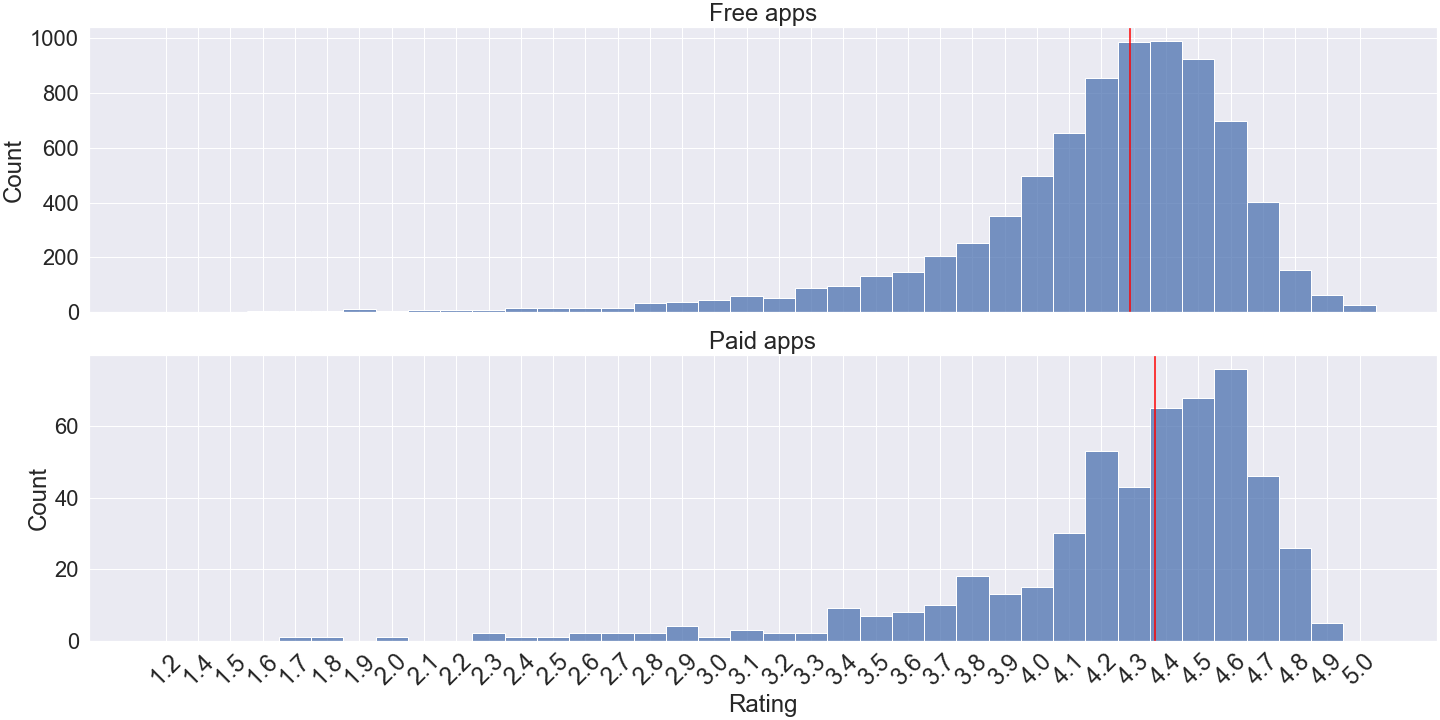
\includegraphics[scale=0.23]{figures/rating_distr.png}
    \caption{Rating distribution of free (top picture) and paid (bottom picture) apps, with corresponding rating mean values across apps given as vertical red lines. Apps with missing rating values or fewer than 20 reviews are not shown. Each bin corresponds to a discrete rating value.}
    \label{fig1}
\end{figure}

As can be seen from this figure, the rating of the vast majority of the apps lies in the range from $2.8$ to $5$. Therefore, for the subsequent analysis, apps with ratings lower than 2.5 will not be considered since they are outliers.

The Kolmogorov-Smirnov test returned a p-value of $1.22\times 10^{-8}$ and a test statistic of $0.138$. The null hypothesis was thus rejected, and both samples were deemed different. This finding together with \cref{fig1} tells us that a paid app is likely to have a slightly higher rating than a free one.

To put this result into a broader context, the average number of installations for free and paid apps was computed. It was found that, on average, free apps are downloaded nearly 175 times more than paid ones. Overall, these results imply that making an app paid can slightly improve its rating, but at the same time this might severely decrease the user base. For that reason, this kind of monetization needs to be well-thought-out by the development team.


\subsection{Relationship between app rating and other features}
\label{other_features}

As a further step, the study aimed to find whether there exists a relationship between the rating of an app and some of its other features. To this end, the app size, price, number of installations, and last updated date were considered and compared to the app rating. \cref{fig2} visualizes the findings. 

\begin{figure}[ht]\centering
\subfloat[App rating vs. price]{\label{a}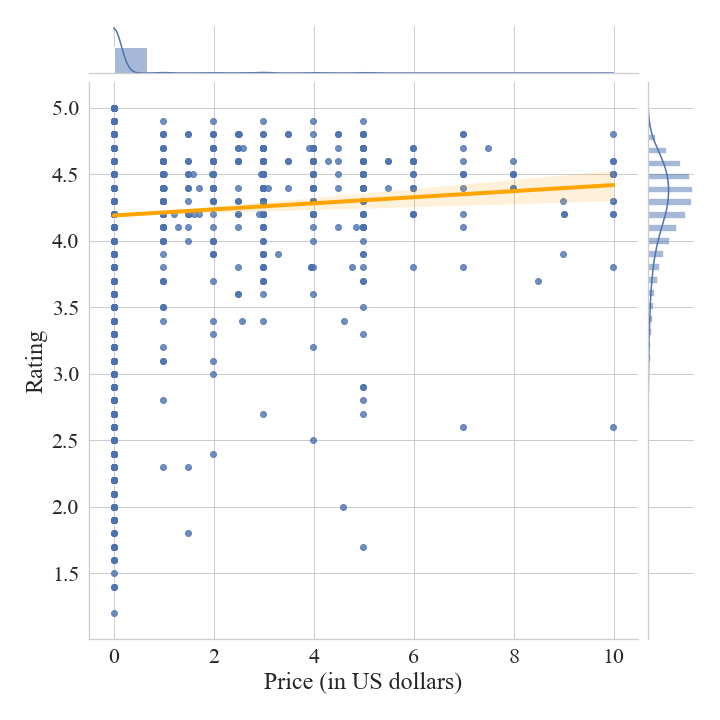
\includegraphics[width=.45\linewidth]{figures/price.png}}\hfill
\subfloat[App rating vs. size]{\label{b}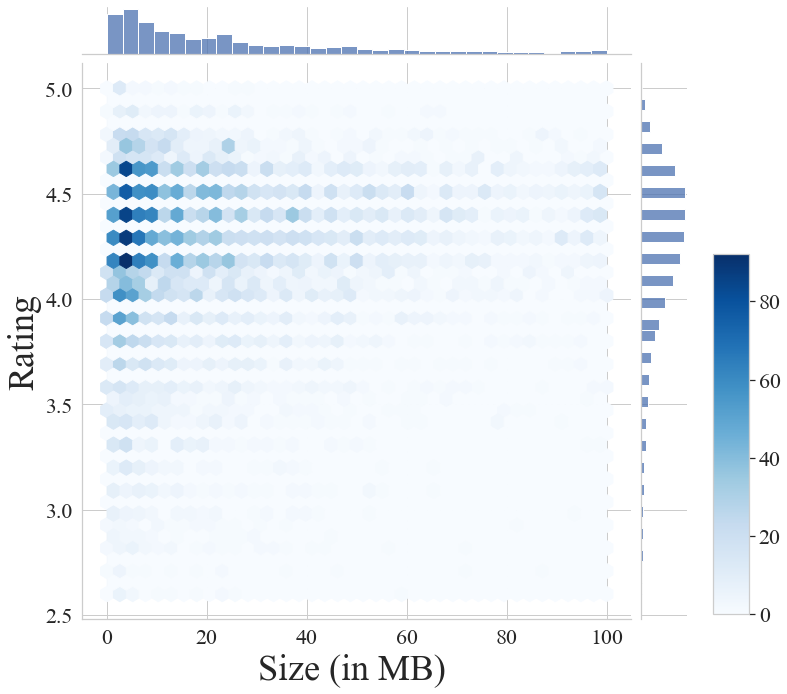
\includegraphics[width=.48\linewidth]{figures/size.png}}\par
\subfloat[App rating vs. number of installations]{\label{c}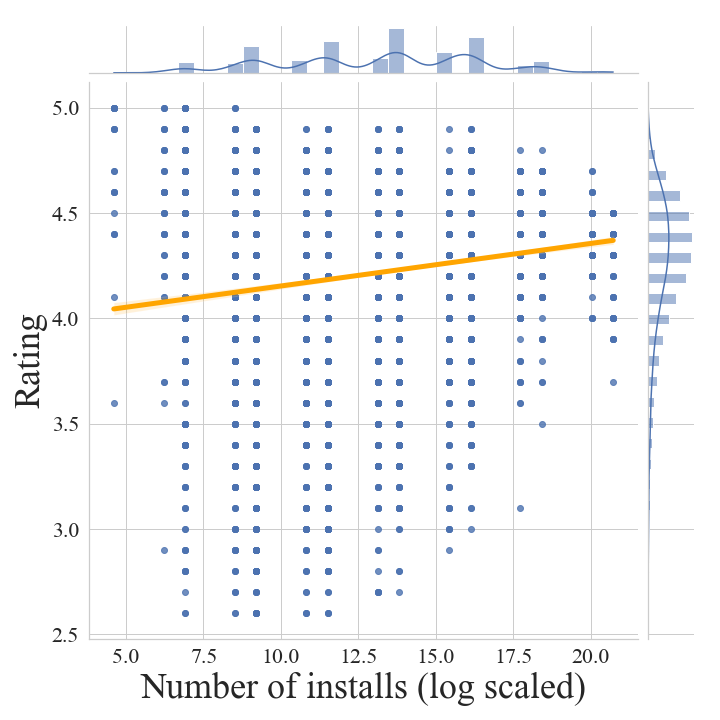
\includegraphics[width=.45\linewidth]{figures/installs.png}}\hfill 
\subfloat[App rating vs. last updated date]{\label{d}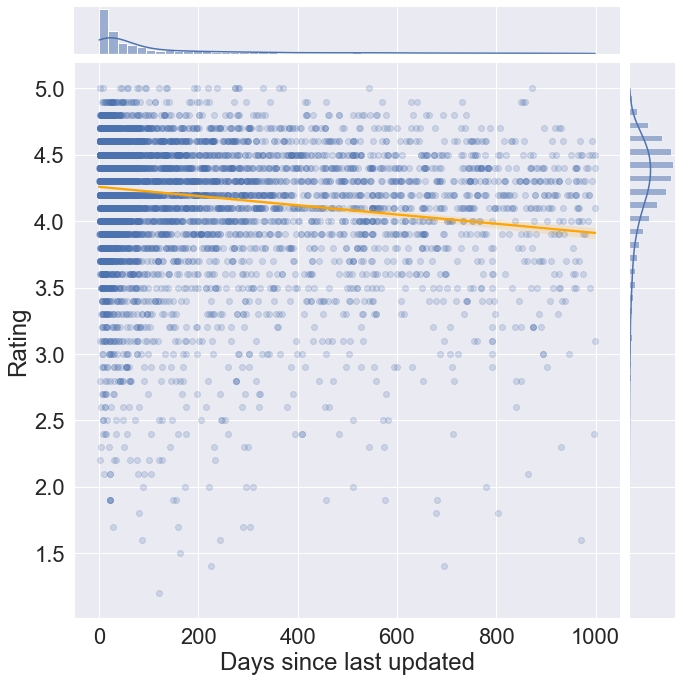
\includegraphics[width=.45\linewidth]{figures/updated.png}}
\caption{The relationship between app rating and app price, size, number of installations and last updated date. In each figure, the top/left plots show the marginal distributions of that feature. Figure (a) compares the app rating to the app price, given in US dollars. Figure (b) shows a density plot of the rating and app size, given in MB. Darker values correspond to higher density. Figure (c) compares the app rating to the log-transformed number of installations. Figure (d) compares the app rating to the last updated date. Orange lines in figures (a), (c) and (d) show the best fitting line found by a standard linear regression model.}
\label{fig2} 
\end{figure}

For all the above features, a standard linear regression model was used to determine a correlation. For the app price, the number of installations, and last updated date, the best fitting line found was plotted in \cref{fig2} as an orange line. As for the app size, no strong relationship could be found. Because of this, only a density plot is shown. 

Choosing a higher price for an app may have a beneficial influence on its rating. This result is not surprising by itself, as users who buy an app have likely done some research on it. Thus, the app price needs to be justified in order for an app to be profitable. Apps that are updated more frequently receive substantially higher ratings. This finding confirms a result found in \cite{freshapps} and can be explained by the fact that apps updated more often have fewer defects and are less prone to security issues. As for the number of installations, the presumed relationship is two-sided - popular apps receive higher ratings and some high-rated apps are likely popular. This finding is expected since teams that can afford big advertising or have a good app idea also have the capacity to ensure high app quality.  The app rating is not strongly affected by its size, implying that users give less weight to size in their reviews compared to other features. This can be also explained by the increase in mobile device storage, which has caused users to worry less about the size of an app. 

\subsection{Limitations and further research}

We found two limitations in this study that could be addressed in future research. First, since paid apps are affordable to fewer people, their ratings are biased by the user profile and the perception of the quality of these users. Further, the number of installations and the rating are imperfect measures of app quality or profitability, since they do not tell, e.g., how long the app was installed or if the ratings were honest or objective. One way to improve on this would be to use sentiment analysis to look at user reviews, which could then give a clearer picture of where an app's shortcomings lie. Based on the results of this study it can be conjectured that, given enough (external) features, an app's rating can be almost perfectly predicted, even without knowing its content or actual quality.

\section{Conclusion}

In this study, we analyzed and visualized app data from the Google Play Store to find out how user ratings are related to other app features. It was found that paid applications receive slightly higher ratings, but also receive less popularity. App rating increases with the price, number of installations and update frequency, while it is not affected by app size. Some limitations of the data, applications and extensions of the analysis were pointed out.

\appendix
\printbibliography


\end{document}